\section{Introduction}
\label{sec:intro}

An LLM agent that operates over days cannot keep everything in context. Since
Generative Agents \citep{park2023generative}, the standard answer to the question of what to store has been to ask the model
itself: rate the importance of each candidate memory and keep the top-rated
ones. Variants of this reflection-based admission
control run inside most deployed agent memory stacks
\citep{packer2023memgpt, zhong2023memorybank}. The practice rests on an assumption that has never been tested under
experimental control of content provenance: that a model's verbal report of
what is important tracks what will actually be useful.

We test this assumption under experimental control of content provenance and
find that it fails for the content that memory selection most needs to capture. We construct episodic
benchmarks in which the single most useful item is either (i) stated explicitly in
the text, or (ii) a silent inference: a bridge concept (``the city is Madrid'') that the model can be shown to carry while reading (\S\ref{sec:causal}) but that never appears
as a word and is required only later, when a probe question arrives (in the
construct-valid designs the bridge is also never the answer itself,
\S\ref{sec:setup}). Asked which concepts are worth remembering, models at every scale we tested
(0.5B--7B) and at every post-training stage (SFT, DPO, RLVR) confidently
nominate vivid, useless surface words and reject the silent bridge: on the
sparse-cue construct-valid benchmarks, verbal importance is at or below
chance as a ranking signal (AUC $0.17$--$0.49$; Table~\ref{tab:master};
Fig.~\ref{fig:hero}). The same reports are good when the useful content is
explicit, better there than any internal signal we test. The failure is robust to probe wording, to the canonical 1--10 rating form,
and to letting the model deliberate before answering; its one measured
boundary is cue density, summarized in \S\ref{sec:dissociation} and mapped
in Appendices~\ref{app:vrobust} and~\ref{app:replications}.

The model knows more than it tells: the information is present in its
internal state but not in its report.
Building
on the J-lens ``workspace'' construction of \citet{anthropic2026workspace}, we read
each concept's availability directly off the residual stream at the end of
encoding: the peak reciprocal rank of the concept's token across layers under the
logit lens \citep{nostalgebraist2020logitlens}. This readout ranks the silently inferred bridges that self-report rejects
above the competing candidates (AUC $0.62$--$0.67$ at 7--8B across four model
families, including the latest Qwen3), is not explained by surface presence, embedding relevance, or
prompt wording (App.~\ref{app:vrobust}), and is causally load-bearing: steering the
bridge's input-side direction while the model answers from memory changes the
answer far more often than a sham direction ($0.70$ vs.\ $0.05$ flip rate at
7B at the gentlest tested scale, $0.60$ vs.\ $0.10$ at 3B;
Table~\ref{tab:causal}).

\updatedparagraph{Downstream, gating memory on the workspace score costs zero
probe passes. The workspace-only arm reaches the selection-oracle accuracy at
7B on the construct-valid benchmark ($0.525$ vs.\ $0.525$) and reaches $0.75$
recall-QA at 0.5B on Evoked. These workspace and oracle arms do not consume
the migrated verbal score; historical direct comparisons against verbal
selected sets are retained as prior evidence and are not used as corrected-v3
headline claims. Full policy comparisons are in \S\ref{sec:prgresults}.}
Finally, the failure is repairable: the reporter never learned to read the
workspace. \updated{On Qwen3-8B, self-distillation from frozen workspace
rankings increases held-out Decoupled verbal AUC by $+0.1642$, $+0.2868$, and
$+0.1873$ across three independently locked seeds (mean $+0.2128$), while
workspace AUC changes by less than $0.001$. Separately, a probe-blind RL-QA
objective learns the admission decision directly from future QA utility and
improves budget-2 recall by $+5.88$ to $+8.82$ points across the same three
8B seeds.} These two additions repair different interfaces: what the model
says is worth remembering, and what the agent actually stores.

\updatedparagraph{\textbf{Revision scope.} The original architecture,
training-free workspace gate, causal intervention, mechanism analyses, and
figures are retained. The new experiments add a corrected 24-checkpoint
log-space measurement grid, a five-size Qwen3 scale ladder, multi-seed
Qwen3-8B Alignment and RL-QA, and exploratory 14B/32B boundary runs. Updated
v3 tables supersede the corresponding pre-migration verbal-score numbers;
workspace-only causal and gating arms are unaffected.}

\textbf{Contributions.}
\textbf{(1)}~A content-provenance regime map for LLM introspective salience:
verbal importance reports are reliable for explicit content and fall at or
below chance for construct-valid silently inferred content, replicated across
four model families (including the latest Qwen3 generation) and three probe wordings, with episode-cluster bootstrap
statistics and a machine analogue of metacognitive efficiency
(\S\ref{sec:setup}, \S\ref{sec:results}). We release the four
provenance-controlled benchmarks, show that existing naturalistic benchmarks
structurally cannot exercise the silently inferred regime
(App.~\ref{app:locomo}), and map the regime's boundary with a measured
cue-density analysis across three generators (App.~\ref{app:replications}).
\textbf{(2)}~A training-free workspace write gate, the first use of a
J-lens-style readout as a write-admission signal, with causal evidence that
memory-based answers read the patched workspace content and budgeted-recall
payoff up to selection-oracle level at zero probe cost; a provenance-routed
extension (PRG) covers mixed streams at tight budgets (\S\ref{sec:method},
\S\ref{sec:prgresults}).
\textbf{(3)}~A post-training diagnosis: in our stage sweep, none of 11 transitions
(8 Qwen base$\to$instruct pairs; OLMo-2 SFT$\to$DPO$\to$RLVR) improves the
workspace channel, and the verbal channel's miscalibration, already present in
raw-probed base models, persists or worsens; we propose and validate
metacognitive alignment, a self-distillation procedure that repairs the verbal
channel, in two model families (\S\ref{sec:extensions}).
\textbf{(4)}~A boundary analysis showing what the static workspace does and does
not hold: a trained future-token lens cannot rescue compositional (two-hop)
bridges, but a utility-gradient readout, the infinitesimal version of our
causal intervention, can in the Qwen family (paired $+0.125$ over the static
readout at 7B; family-dependent, \S\ref{sec:extensions},
App.~\ref{app:family}).
\updatedparagraph{\textbf{(5)}~A scaled and multi-seed extension that separates two
repair targets: workspace-derived self-distillation calibrates the verbal
reporter, whereas probe-blind RL-QA learns the memory action without observing
the workspace probe (\S\ref{sec:newexperiments}).}

\begin{figure}[t]
\centering
\IfFileExists{figures/intro.png}{%
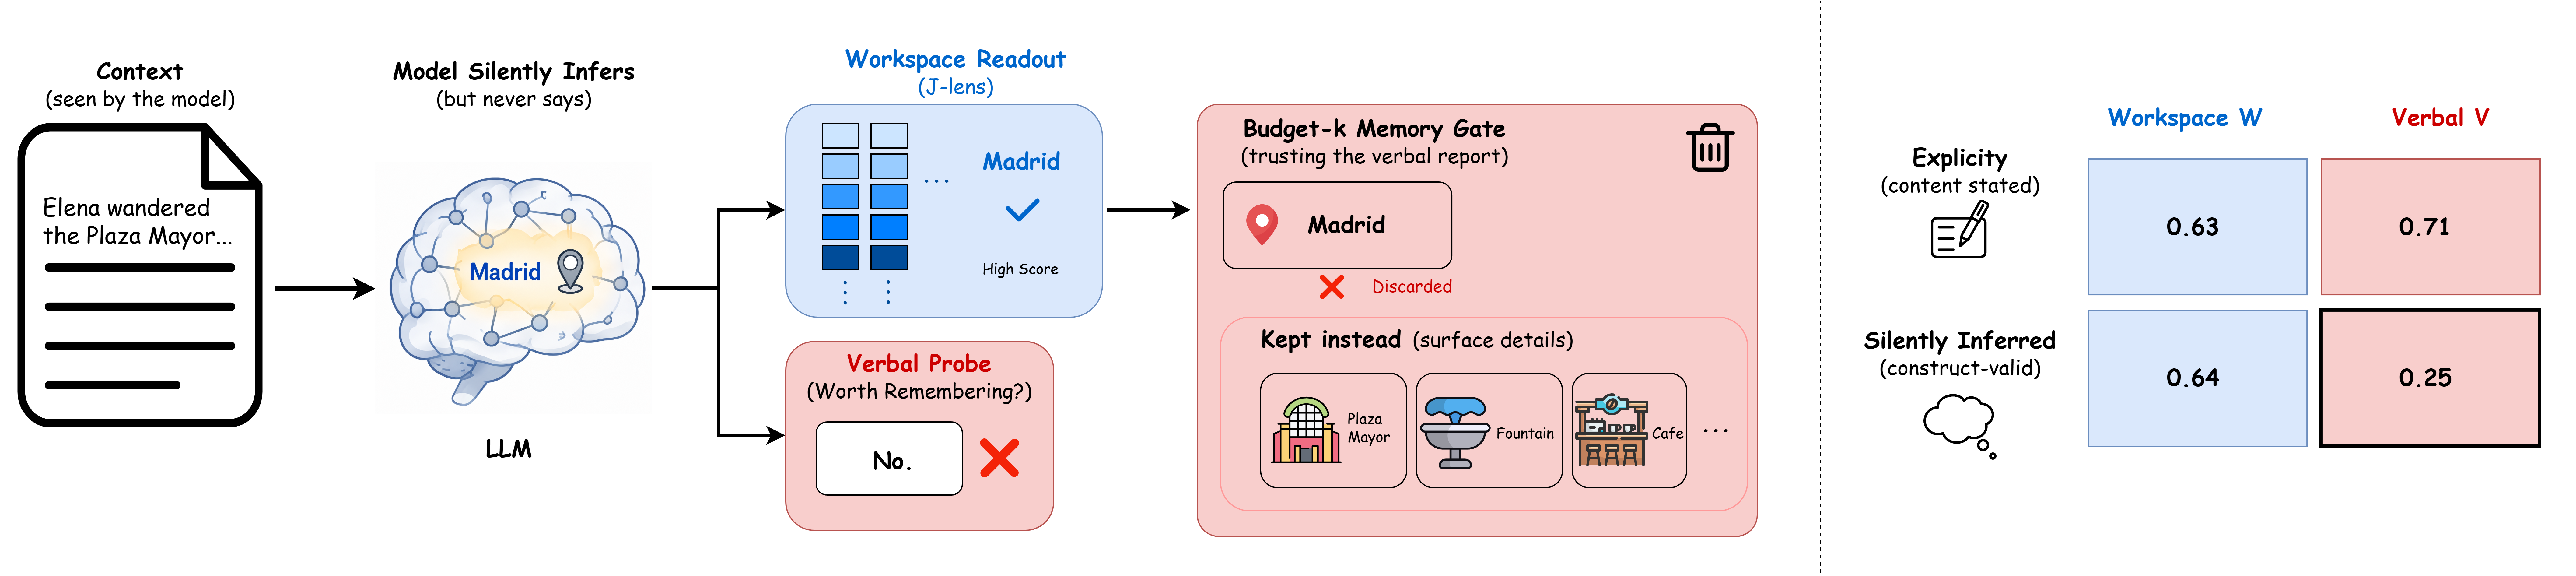
\includegraphics[width=\textwidth]{figures/intro.png}}{%
\fbox{\parbox[c][4.6cm][c]{0.96\textwidth}{\centering
\emph{Hero figure (figures/fig1\_hero.pdf).}\\[4pt]
\textbf{Left:} write-gating schematic. Context ``Elena wandered the Plaza
Mayor\ldots'' $\rightarrow$ model silently infers \emph{madrid} (high in the
J-lens workspace readout $\checkmark$) but rates it unimportant verbally
($\times$) $\rightarrow$ budget-$k$ gate on the verbal report drops the item
needed for ``What language should Elena use?''.\\[4pt]
\textbf{Right:} $2\times2$ AUC heatmap, regime (explicit / inferred)
$\times$ channel (workspace $W$ / verbal $V$), showing the dissociation:
$V$ wins on explicit, is anti-calibrated on inferred; $W$ the reverse.}}}
\caption{\textbf{Left:} the write-gating problem. Reading ``Elena wandered the
Plaza Mayor\ldots'', the model silently infers \emph{madrid}, and the inference
is visible in a J-lens-style workspace readout of its residual stream; asked
whether \emph{madrid} is worth remembering, it confidently says no. A budget-$k$ memory gate
that trusts the verbal report discards exactly the item needed to answer ``What
language should Elena use?''. \textbf{Right:} AUC of each channel at identifying
truly load-bearing items (Qwen-3B shown; same qualitative dissociation at
3B--7B in all four families, with knife-edge small-scale cells noted in
App.~\ref{app:prereg};
Table~\ref{tab:master}): the verbal report is good for explicit content but
below chance for construct-valid silently inferred content (boxed cell;
generator analysis in \S\ref{sec:dissociation}); the workspace readout is
not.}
\label{fig:hero}
\end{figure}
